\documentclass[11pt]{article}

% ---------------------------------------------------------------------------
% Build switch.  \anonfalse = named preprint (arXiv).
%                \anontrue  = anonymised build for CHIL double-blind review.
% ---------------------------------------------------------------------------
\newif\ifanon
\anontrue

\usepackage[a4paper,margin=2.5cm]{geometry}
\usepackage{times}
\usepackage[T1]{fontenc}
\usepackage[utf8]{inputenc}
\usepackage{amsmath,amssymb}
\usepackage{booktabs}
\usepackage{graphicx}
\usepackage{caption}
\usepackage{authblk}
\usepackage[hidelinks]{hyperref}
\usepackage{microtype}
\usepackage[numbers,sort&compress,square]{natbib}

\captionsetup{font=small,labelfont=bf}
\setlength{\parskip}{0pt}
\renewcommand{\arraystretch}{1.12}

\title{\vspace{-1.5em}\bfseries Character accuracy conceals numerical error:\\
measuring silent value corruption in a clinical document pipeline}

\ifanon
  \author[ ]{}
  \affil[ ]{\small Author details withheld for double-blind review}
\else
  \author[ ]{Mohammed Jabir Hussain Shaik}
  \affil[ ]{\small School of Electronics, Electrical Engineering and Computer Science\\
  Queen's University Belfast, United Kingdom\\
  \texttt{mshaik01@qub.ac.uk}}
\fi
\date{}

\begin{document}
\maketitle

\begin{abstract}
\noindent
Clinical decision support systems increasingly read patient data from document images, where
optical character recognition sits between the page and every downstream inference. Reported
accuracy for that stage is usually character-level, and a laboratory value is not a character.
We measured the image-to-value path of a retrieval-based clinical decision support prototype
under controlled image degradation, using synthetic reports carrying exact machine-readable
ground truth for 13 analytes, with the document as the experimental unit across 10 independent
reports and 7 scan resolutions. At 100~dpi, character accuracy remained at
88.9\% while 32.3\% of laboratory values were misread and a further
10.0\% were not read at all. Of 188 corrupted values, 89 (47.3\%)
carried the same abnormality flag as the true value, leaving the error invisible to the
alerting layer. We identify the mechanism: because abnormality flags are threshold
quantisations, corruption of a value that was already outside its reference range is
substantially more likely to preserve the flag than corruption of a normal value
(61.7\% against 22.1\%, Fisher exact $p = 1.6 \times 10^{-7}$,
odds ratio 5.68). Fourteen of fifteen corrupted troponin readings were hundredfold
overstatements that retained the \emph{Critical} flag. A physiological plausibility bound
rejected 104 of 188 corruptions and recovered 33 of the 89 silent ones, failing entirely for
analytes whose plausible range is wide relative to their reference range. Substituting a
large language model for the deterministic extractor repaired nothing. These findings come
from synthetic documents and one OCR engine, and they bound no claim about real clinical
performance; what they do establish is that character-level accuracy is not a safety metric
for pipelines that reduce measurements to flags.
\end{abstract}

\section{Introduction}

A clinical decision support system that reads a patient record from a scanned page performs a
chain of inferences before any model reasons about the patient. Pixels become characters,
characters become a labelled value, the value is compared against a reference range, and the
resulting flag reaches the clinician or the generator. Each step can fail, and the failures do
not announce themselves in the same way.

Work on retrieval-augmented generation in healthcare has concentrated on what happens after a
value exists: whether the right passage is retrieved, whether the answer is grounded, whether a
citation points where it claims to \citep{gao2023rag,amugongo2025rag,lu2024clinicalrag}. That
literature assumes the number arriving from the document is the number printed on it. When the
document is a photograph or a fax, the assumption is doing work that nobody has measured.

Optical character recognition is normally reported through character error rate, and character
error rate treats every symbol as equivalent. A decimal point is one character. In
\texttt{5.8 mEq/L} it is also the difference between a potassium concentration requiring
monitoring and one incompatible with life. A pipeline can therefore post a high character
accuracy and still deliver a wrong number, and the number is what the clinical logic consumes.

We report two experiments on this path. The first sweeps 32 degradation conditions on a single
document to establish which corruptions occur. The second takes the document as the
experimental unit across 10 independent reports and 7 resolutions, and measures how often
values are misread, how often they are lost, and what the system's own flagging layer does with
the result.

Our contributions are the following. We quantify the dissociation between character accuracy
and value accuracy in a clinical extraction pipeline. We give a taxonomy of what corruption
does to an abnormality flag, and show that the most common outcome is no change at all. We
identify the mechanism behind that outcome, which is threshold quantisation, and show it is
predicted by whether the true value was already abnormal. We evaluate a physiological
plausibility bound and characterise where it systematically fails. We report that replacing the
deterministic extractor with a language model repaired no error and introduced none.

\section{Related work}

Retrieval-augmented generation has been proposed widely for clinical question answering, and
recent reviews survey its use across healthcare tasks \citep{gao2023rag,amugongo2025rag}.
Systems such as ClinicalRAG retrieve over heterogeneous clinical knowledge
\citep{lu2024clinicalrag}, and question-answering corpora such as MedQuAD provide evaluation
material \citep{benabacha2019medquad}. These evaluations measure retrieval and generation
quality on text that is already text.

Document-level work in clinical natural language processing generally begins from transcribed
records, and OCR quality is reported, where it is reported, as a character or word error rate.
We are not aware of a study that measures how character-level degradation propagates into
extracted numerical values and then into the abnormality flags that clinical logic acts on,
which is the gap this work addresses.

\section{Methods}

\subsection{Documents and ground truth}

Each synthetic report is generated with a machine-readable truth file recording the exact value,
unit, printed reference range and expected flag for 13 analytes: fasting glucose, HbA1c,
haemoglobin, ferritin, white cell count, platelets, sodium, potassium, blood urea nitrogen,
creatinine, eGFR, troponin I and LDL cholesterol. The panel was chosen to span several orders of
magnitude and several decimal conventions, so that a lost decimal point produces an error of
different size depending on the analyte.

No real patient data were used at any stage.

\subsection{Degradation conditions}

Documents are rendered from PDF at a specified resolution and then degraded. The condition set
covers resolution (300, 200, 150, 120, 100, 85 and 72 dpi), Gaussian blur
($\sigma \in \{0.5, 1.0, 1.5, 2.0, 3.0\}$), JPEG compression (quality
$\in \{90, 70, 50, 30, 15\}$), rotation ($\{0.25, 0.5, 1.0, 2.0, 5.0\}$ degrees), additive
noise ($\{5, 10, 20, 30, 50\}$), and five composites intended to resemble real capture paths:
a good scan, an office scan, a phone photograph, a poor fax and a poor photograph.

Stochastic conditions are run with five seeds. Experiment~1 therefore comprises 24
single-seed conditions and 8 conditions at five seeds each, giving 64 runs and, across 13
analytes, 832 observations on one document.

\subsection{Extraction, flagging and the plausibility bound}

Degraded images are passed to Tesseract (\texttt{--psm 6}). A deterministic parser locates each
analyte by label and extracts the first numeric token on the line.

The flagging logic is transcribed, rather than imported, from the prototype's
\texttt{clinical\_parser} module so that the experiment runs without the application stack. The
transcription preserves a property of the deployed system worth stating plainly: its reference
ranges are fixed, are not age- or sex-aware, and are not the ranges printed on the document. The
system flags haemoglobin outside 12.0--17.5~g/dL while the generated
report prints 12.0--15.5~g/dL.

We additionally implement a physiological plausibility bound, a generous envelope of values
possible in a living patient, and ask whether it would have rejected each corruption. This
envelope is our own construction for this study and is not a clinical standard.

\begin{figure}[t]
\centering
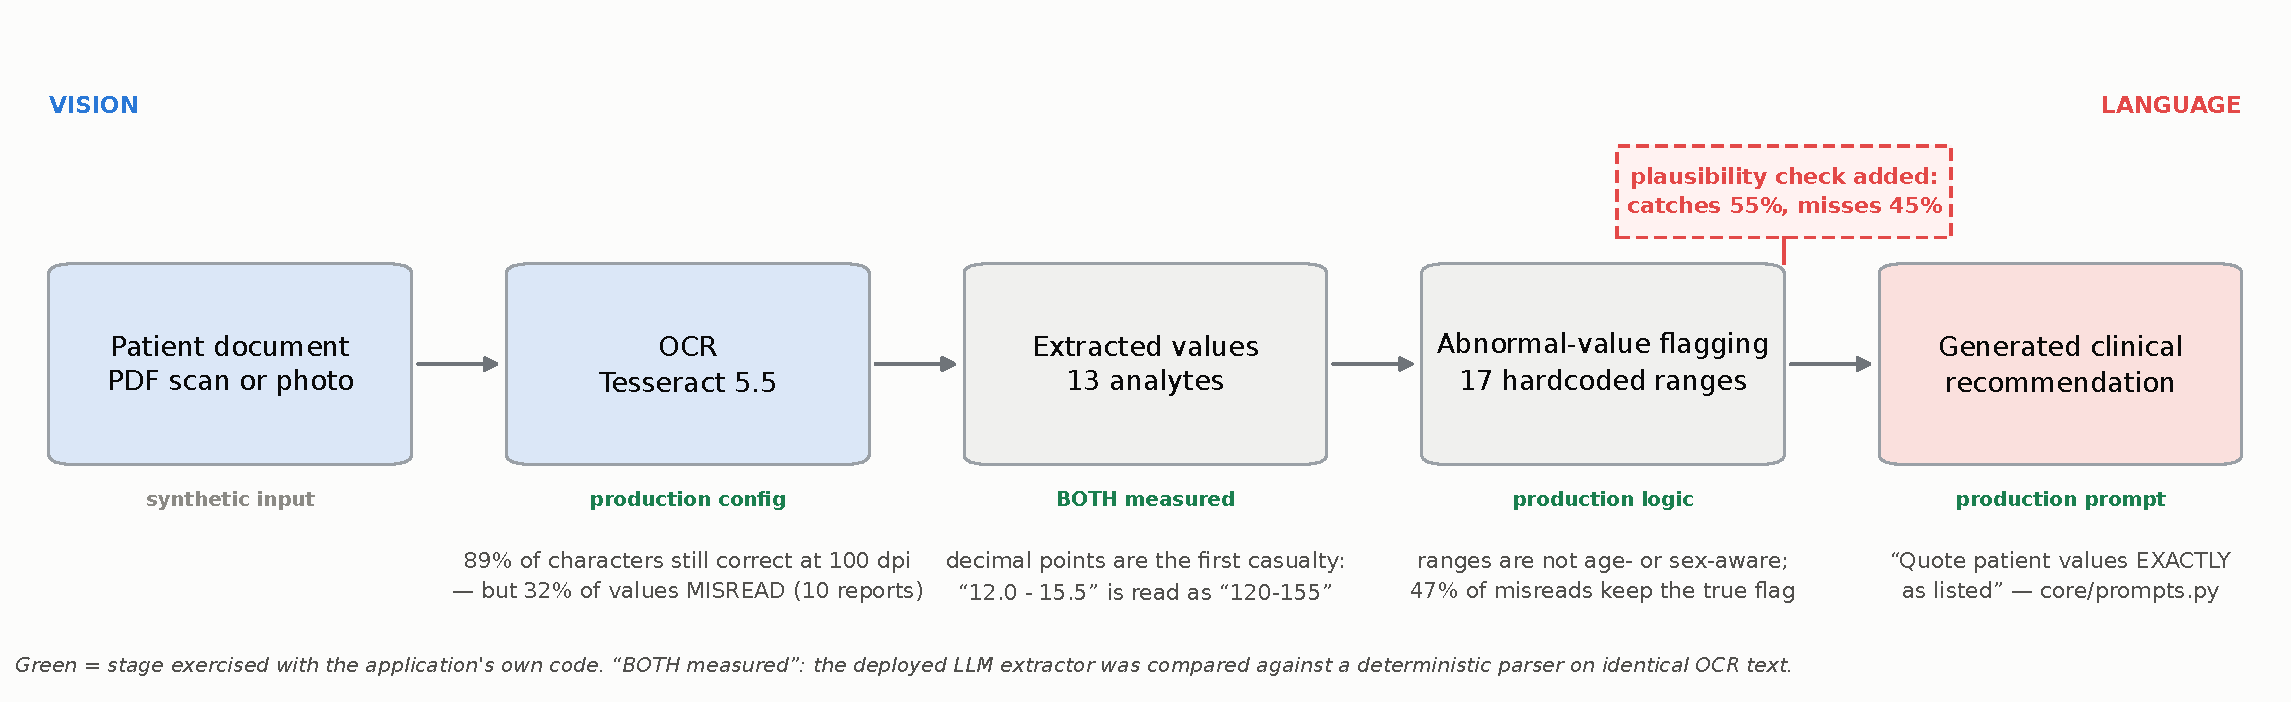
\includegraphics[width=\textwidth]{figures/fig1_architecture.pdf}
\caption{The measured path, with one observed case. A potassium concentration of
5.8~mEq/L printed on the page is extracted as 58.0 and carries the same \emph{High} flag as the
true value. Stages marked in green were exercised using the prototype's own code. The
potassium case is one observed instance from the single-document sweep and is not a frequency.
Whether a corrupted value changes a generated recommendation was not tested.}
\label{fig:pipeline}
\end{figure}

\subsection{Experimental unit and the calibration gate}

Thirteen analytes read from one page are not thirteen independent observations, since they share
a rendering, a scan and an OCR pass. Experiment~2 therefore treats the document as the
experimental unit: proportions are computed within each of 10 independent reports and summarised
across them, and every dispersion we report is a standard deviation between documents rather
than a confidence interval.

No result is reported for a document unless its clean 300~dpi render returns all 13 values
correctly. This gate separates degradation effects from generation or parsing faults. All 10
documents passed.

Experiment~2 comprises 10 documents $\times$ 7 resolutions $\times$ 13 analytes, giving 910
observations.

\subsection{Outcome definitions}

Each reading is \emph{correct}, \emph{misread} (a value was emitted and it differs from truth)
or \emph{unread} (no value was emitted for that analyte). Misread and unread are different
failures with different consequences and we never pool them.

Character error rate is Levenshtein distance between the whitespace-normalised reference text
and the OCR output, divided by the length of the reference.

\section{Results}

\subsection{Which degradations corrupt values, and which destroy them}

Experiment~1 sweeps 32 conditions on one document to establish which failure modes exist before
committing the replicated design to a single axis. Table~\ref{tab:families} gives the outcome by
degradation family.

\begin{table}[t]
\centering
\caption{Experiment~1: outcome by degradation family, 832 observations on one document.
\emph{Corrupted} means a wrong value was emitted; \emph{label not found} means the analyte's line
was not located at all. JPEG compression to quality 15 and rotation to five degrees produced
neither outcome.}
\label{tab:families}
\small
\begin{tabular}{lcccc}
\toprule
Family & Observations & Corrupted (\%) & Label not found (\%) \\
\midrule
Baseline (300~dpi) & 13  & \phantom{0}0.0 & \phantom{0}0.0 \\
JPEG quality 90--15 & 65  & \phantom{0}0.0 & \phantom{0}0.0 \\
Rotation 0.25--5$^\circ$ & 65  & \phantom{0}0.0 & \phantom{0}0.0 \\
Noise 5--50 & 325 & \phantom{0}1.5 & 20.0 \\
Blur $\sigma$ 0.5--3.0 & 65  & \phantom{0}9.2 & \phantom{0}0.0 \\
Composite capture paths & 221 & \phantom{0}6.3 & 56.1 \\
Resolution 200--72~dpi & 78  & 23.1 & 10.3 \\
\bottomrule
\end{tabular}
\end{table}

The families separate by failure mode. Resolution is the dominant source of wrong values.
Noise and the composite capture paths mostly prevent the analyte's label from being located, so
the value is absent rather than wrong. JPEG compression and small rotations produced no error of
either kind at the levels tested.

This distinction matters for risk. An analyte that is not found is an absence a caller can
detect. A misread analyte is a confident wrong answer. Because resolution is the condition that
most readily produces the second case, Experiment~2 replicates the resolution axis across 10
independent documents.

\subsection{Character accuracy and value accuracy separate}

Table~\ref{tab:resolution} gives both measures across the resolution sweep. At 300~dpi no
value was misread in any of the 130 analyte readings. Degradation then affects the two measures
at different rates. Between 300~dpi and 100~dpi, character accuracy falls by
9.2 percentage points while the misread rate rises from zero to 32.3\%.

\begin{table}[t]
\centering
\caption{Character accuracy and value outcomes across the resolution sweep. Each cell is the
mean over 10 independent documents, with the standard deviation between documents in
parentheses. Misread means a wrong value was emitted; unread means no value was emitted.}
\label{tab:resolution}
\small
\begin{tabular}{lccc}
\toprule
Resolution & Character accuracy (\%) & Values misread (\%) & Values unread (\%) \\
\midrule
300~dpi & 98.10 & \phantom{0}0.00 \phantom{(00.00)} & \phantom{0}0.00 \phantom{(00.00)} \\
200~dpi & 98.02 & \phantom{0}1.54 (3.24) & \phantom{0}0.00 \phantom{(00.00)} \\
150~dpi & 96.67 & \phantom{0}4.62 (5.38) & \phantom{0}0.00 \phantom{(00.00)} \\
120~dpi & 96.12 & 12.31 (9.73) & \phantom{0}0.00 \phantom{(00.00)} \\
100~dpi & 88.88 & 32.31 (9.46) & 10.00 (5.19) \\
85~dpi  & 80.83 & 49.23 (13.66) & 14.62 (5.68) \\
72~dpi  & 56.53 & 44.62 (21.08) & 41.54 (27.43) \\
\bottomrule
\end{tabular}
\end{table}

\begin{figure}[t]
\centering
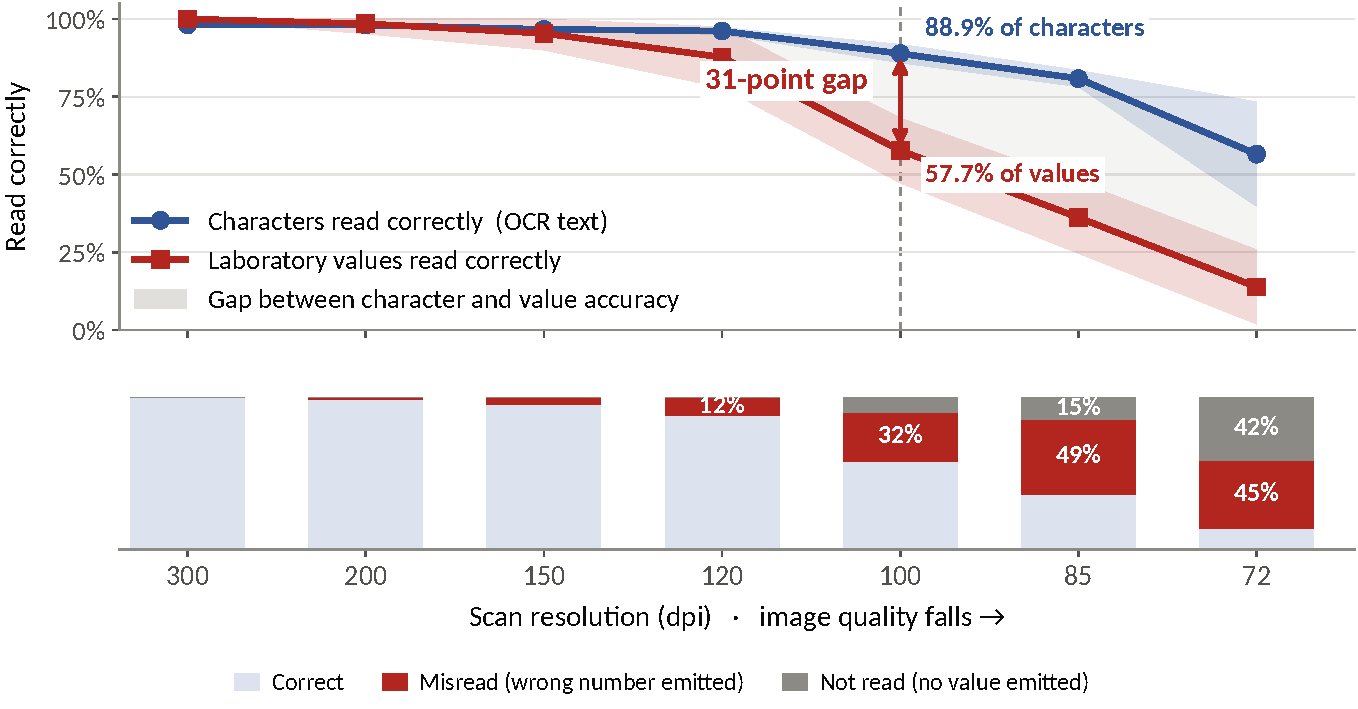
\includegraphics[width=\textwidth]{figures/fig2_resolution_paper.pdf}
\caption{Character accuracy and value accuracy across the resolution sweep. Each point is the
mean over 10 independent documents and bands are $\pm1$ standard deviation between documents,
not confidence intervals. The lower panel decomposes each resolution into values read correctly,
values misread, and values not read. At 100~dpi the two measures differ by 31 percentage points.}
\label{fig:resolution}
\end{figure}

Below 85~dpi the misread rate stops rising while the unread rate more than doubles. Paired
by document between 85~dpi and 72~dpi, the misread rate fell for four documents, rose
for three and was unchanged for three (mean change $-4.6$ percentage points, SD 20.9). The data
are consistent with values ceasing to be read rather than being read wrongly, and they do not
establish a decrease.

\subsection{What corruption does to the flag}

Across Experiment~2, 188 of 910 readings were misread. Table~\ref{tab:taxonomy} classifies each
by what happened to the abnormality flag. The largest category is no change: 89 corruptions
(47.3\%) produced a value that carried the same flag as the truth. For those
readings the error is invisible to any component that consumes the flag rather than the value.

\begin{table}[t]
\centering
\caption{What corruption did to the abnormality flag, for all 188 misread values in
Experiment~2. Categories are mutually exclusive. The silent share computed within each document rather than pooled gives a mean of 48.2 percent (SD 12.7, range 23 to 64 across the 10 documents).}
\label{tab:taxonomy}
\small
\begin{tabular}{lcc}
\toprule
Outcome & Count & Share of corruptions (\%) \\
\midrule
Flag unchanged (silent)                 & 89 & 47.3 \\
Normal value flagged abnormal           & 53 & 28.2 \\
Flag changed, wrong direction or severity & 41 & 21.8 \\
Abnormal value read as normal           & \phantom{0}5 & \phantom{0}2.7 \\
\midrule
Total                                   & 188 & 100.0 \\
\bottomrule
\end{tabular}
\end{table}

\subsection{Already-abnormal values hide their own corruption}

The silent category is not distributed at random. Splitting the 188 corruptions by whether the
true value was already outside its reference range gives 61.7\% silent among the
120 corruptions of abnormal values, against 22.1\% among the 68 corruptions of
normal values (Figure~\ref{fig:mechanism}; Fisher exact $p = 1.6 \times 10^{-7}$, odds ratio 5.68).

The mechanism is structural rather than incidental. An abnormality flag is a threshold
quantisation of a continuous measurement. Once a value lies outside its reference range, moving
it further outside does not change which side of the threshold it falls on. Corruption that
crosses a threshold is detected by the flagging layer; corruption that drives an already
abnormal value deeper into abnormality is invisible by construction.

\begin{figure}[t]
\centering
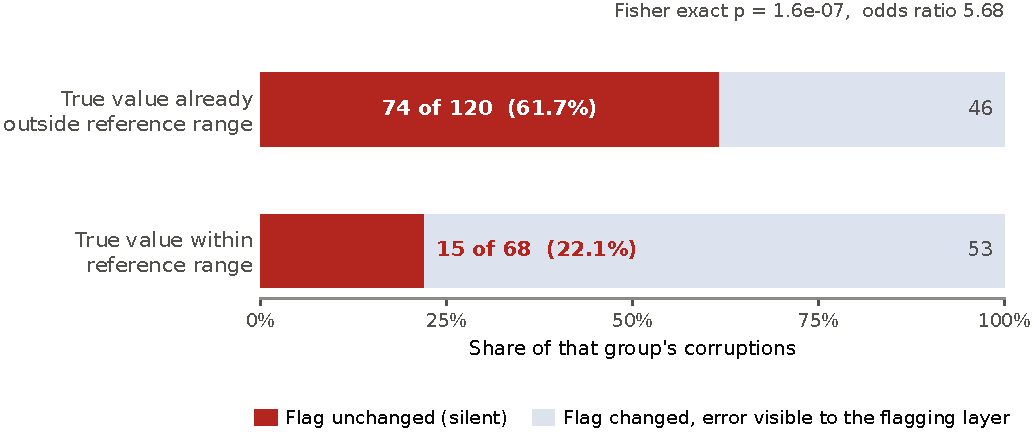
\includegraphics[width=0.92\textwidth]{figures/fig3_mechanism.pdf}
\caption{Corruption of a value that was already outside its reference range is far more likely
to leave the abnormality flag unchanged. Bars show, within each group, the share of that group's
corruptions that were silent. All 188 corruptions from Experiment~2 are included and the two
groups are disjoint.}
\label{fig:mechanism}
\end{figure}

Decimal-shift errors make the same point quantitatively. Of 188 corruptions, 102
(54.3\%) were decimal shifts, all of them upward. Tenfold shifts
($n = 87$) were silent in 42.5\% of cases, while hundredfold shifts ($n = 15$) were
silent in 86.7\%. The larger error is the more invisible one.

Troponin I illustrates the consequence. Fourteen of its fifteen corrupted readings were
hundredfold overstatements, and every one retained the \emph{Critical} flag:
0.07~ng/mL read as 7.0, 0.82 read as 82.0. A
borderline result and a result two orders of magnitude higher are indistinguishable downstream.

\subsection{A plausibility bound helps, and fails systematically}

The plausibility bound rejected 104 of the 188 corruptions (55.3\%) and rejected
none of the 636 correct values. The absence of false positives is guaranteed by the generator,
which samples truth values strictly inside the envelope, and is not an estimate of a real
false-positive rate.

Of the 89 silent corruptions, the bound recovered 33 (37.1\%), leaving 56 that
neither the flagging layer nor the plausibility check would surface.

Per-analyte detection ranges from 96.9\% for potassium to zero for troponin I,
ferritin, fasting glucose and eGFR (Table~\ref{tab:peranalyte}). We tested whether detection is
predicted by the ratio of plausible envelope width to reference range width. The association is
in the expected direction and does not reach significance at this sample size
(Spearman $\rho = -0.48$, $p = 0.09$, $n = 13$), and eGFR contradicts it: its envelope is the
narrowest of the panel relative to its reference range, yet no corruption was detected, because
the envelope's lower bound is zero and every observed eGFR corruption moved the value downward.
Detectability depends on where a corrupted value lands relative to an envelope boundary, which
is not captured by width alone.

\begin{table}[t]
\centering
\caption{Plausibility-bound detection rate per analyte, over the corruptions observed for that
analyte in Experiment~2. Analytes whose plausible envelope is wide relative to their reference
range, or whose envelope is open at the relevant end, are not protected.}
\label{tab:peranalyte}
\small
\begin{tabular}{lcc}
\toprule
Analyte & Corruptions & Detected (\%) \\
\midrule
Potassium          & 32 & 96.9 \\
Haemoglobin        & 33 & 90.9 \\
Sodium             & \phantom{0}6 & 83.3 \\
Platelets          & 16 & 75.0 \\
HbA1c              & \phantom{0}4 & 75.0 \\
Creatinine         & 27 & 59.3 \\
Blood urea nitrogen & \phantom{0}7 & 42.9 \\
White cell count   & 18 & 16.7 \\
LDL cholesterol    & \phantom{0}8 & 12.5 \\
eGFR               & \phantom{0}8 & \phantom{0}0.0 \\
Fasting glucose    & \phantom{0}8 & \phantom{0}0.0 \\
Ferritin           & \phantom{0}6 & \phantom{0}0.0 \\
Troponin I         & 15 & \phantom{0}0.0 \\
\bottomrule
\end{tabular}
\end{table}

\subsection{A language model extractor repaired nothing}

We replaced the deterministic parser with a language model extractor (Llama 3.2 3B via Ollama,
temperature 0) and ran both over identical OCR text across 12 conditions at two repeats. In
four of the 24 runs the model returned no values at all after emitting malformed JSON
(\texttt{rotate\_5.0} twice, \texttt{noise\_30} twice). Over the 260 readings from the 20 runs
that returned values, both extractors were correct on the same 188: zero repairs and zero new
errors.

The corruption is established before either extractor sees the text, and a model reading the
same damaged characters reproduces the same damaged number.

\section{Discussion}

The practical consequence is that character-level accuracy does not bound value-level risk in a
pipeline of this shape. A system reporting 88.9\% character accuracy was delivering
wrong values for roughly a third of the panel, and for nearly half of those the downstream
alerting layer could not tell.

Threshold quantisation is common in clinical software, because reference ranges and severity
bands are how laboratory results are presented. The finding here is that quantisation is also an
information-destroying step placed immediately after an error-prone one. Any check that operates
on the flag rather than the value inherits a blind spot whose size depends on how abnormal the
true value was. The patients whose values are furthest outside the reference range are the
patients whose corrupted readings are hardest to detect.

The plausibility bound is worth implementing and is not sufficient on its own. It is cheapest
where it is least needed, for analytes like potassium whose physiological envelope is narrow,
and it provides nothing for analytes like troponin whose plausible range spans several orders of
magnitude.

Two mitigations follow from the mechanism rather than from the specific numbers. Carrying a
magnitude check alongside the flag, for example a comparison against the range printed on the
document itself rather than a hardcoded range, would detect errors the flag cannot. Treating
unread and misread differently matters as well: an unread analyte is an absence a caller can
notice, while a misread one is a confident wrong answer.

\section{Limitations}

The documents are synthetic. They carry exact ground truth, which is what makes the measurement
possible, and they are not real clinical documents. Nothing here establishes a rate for any
deployed system, and no clinician reviewed any output.

One OCR engine was used, at one page segmentation mode, with one document layout and one panel
of 13 analytes. Every quantity we report is conditional on that stack.

Resolution and pixels per glyph are entangled, since body text varies between 8.5 and 10 point
across the generated documents. A reader could reasonably hold that character size in pixels,
rather than nominal resolution, is the operative variable, and this design cannot separate them.

The plausibility envelope is our construction. Its zero false-positive rate is an artefact of a
generator that samples inside it.

The degradation sweep in Experiment~1 and the extractor comparison use a single document. Only
the resolution sweep is replicated across 10 documents, and only the resolution results carry
between-document dispersion.

We did not measure whether a corrupted value changes a clinical recommendation. The propagation
of a corrupted value into generated text was observed on one document and is not quantified
here.

\section{Conclusion}

Character accuracy and value accuracy come apart under degradation, and the gap is widest
exactly where the clinical stakes are highest. Nearly half of the value corruptions we observed
preserved the abnormality flag, and corruption of an already-abnormal value was more than five
times as likely to be silent as corruption of a normal one, because a threshold cannot represent
how far past it a value has moved. A plausibility bound recovers some of this and fails
systematically for the analytes with the widest physiological ranges. Substituting a language
model for a deterministic parser changed nothing, because the information was lost before either
could read it. Knowing where a number came from is not the same as knowing it was read
correctly.

\section*{Data and code availability}

\ifanon
The experiment scripts, generated documents, truth files, raw OCR output and all result tables
are provided through an anonymised repository link with the submission. Synthetic data are used
throughout; no real patient information was processed at any stage.
\else
The experiment scripts, generated documents, truth files, raw OCR output and all result tables
are available in the project repository. Synthetic data are used throughout; no real patient
information was processed at any stage.
\fi

\section*{Institutional review board}

The research does not require IRB approval. It uses only synthetic documents generated for this
study and involves no human subjects, human tissue or identifiable personal data.

\section*{Statement on AI use}

An AI assistant was used for manuscript drafting and editing, and for exploratory discussion of
analysis options. All experiments, code, analysis and verification were performed by the author.
Every numerical claim in this paper was independently recomputed from the raw result files
before submission.

\begin{thebibliography}{9}
\small

\bibitem[Amugongo et al.(2025)]{amugongo2025rag}
Amugongo, L. M., et al. (2025).
Retrieval augmented generation for large language models in healthcare: a systematic review.
\emph{PLOS Digital Health}, 4(6), e0000877.

\bibitem[Ben Abacha and Demner-Fushman(2019)]{benabacha2019medquad}
Ben Abacha, A., and Demner-Fushman, D. (2019).
A question-entailment approach to question answering.
\emph{BMC Bioinformatics}, 20, 511.

\bibitem[Gao et al.(2023)]{gao2023rag}
Gao, Y., et al. (2023).
Retrieval-augmented generation for large language models: a survey.
\emph{arXiv:2312.10997}.

\bibitem[Lu et al.(2024)]{lu2024clinicalrag}
Lu, Y., Zhao, X., and Wang, J. (2024).
ClinicalRAG: enhancing clinical decision support through heterogeneous knowledge retrieval.
In \emph{Proceedings of the KnowLLM Workshop, ACL 2024}, pp. 64--68.

\end{thebibliography}

\end{document}
